%
% graph.tex
%
% (c) 2019 Prof Dr Andreas Müller, Hochschule Rapperswil
%
\documentclass[tikz]{standalone}
\usepackage{amsmath}
\usepackage{times}
\usepackage{txfonts}
\usepackage{pgfplots}
\usepackage{csvsimple}
\usetikzlibrary{arrows,intersections,math}
\begin{document}

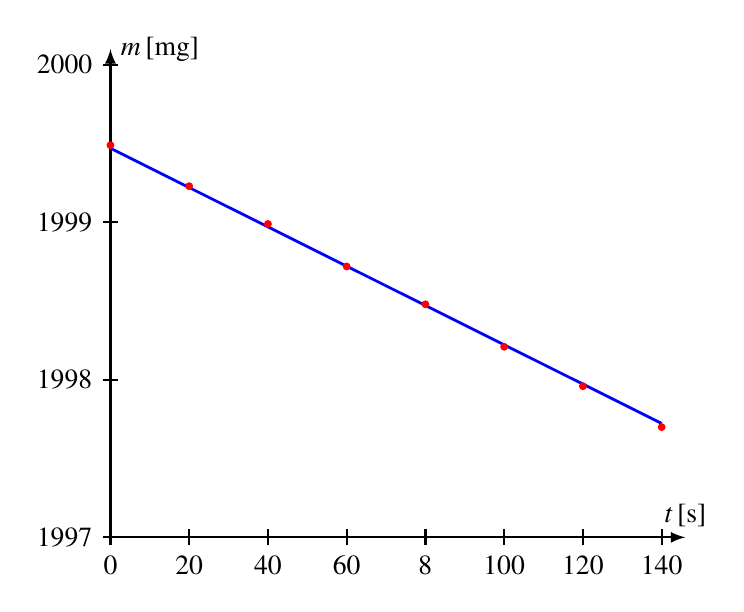
\begin{tikzpicture}[>=latex,thick]
\draw[->] (0,-0.1)--(0,6.2) coordinate[label={right:$m\,\text{[mg]}$}];
\draw[->] (-0.1,0)--(7.3,0) coordinate[label={$t\,\text{[s]}$}];

\def\punkt#1#2{
	\fill[color=red] ({#1/20},{2*(#2-1997)}) circle[radius=0.05];
}

\def\a{-0.0124767}
\def\b{2.470872}

\draw[color=blue,line width=1pt] (0,{2*\b})--(7,{2*(\a*140+\b)});

\punkt{  0.0}{1999.49}
\punkt{ 20.0}{1999.23}
\punkt{ 40.0}{1998.99}
\punkt{ 60.0}{1998.72}
\punkt{ 80.0}{1998.48}
\punkt{100.0}{1998.21}
\punkt{120.0}{1997.96}
\punkt{140.0}{1997.70}

\draw (-0.1,2)--(0.1,2);
\draw (-0.1,4)--(0.1,4);
\draw (-0.1,6)--(0.1,6);

\node at (-0.1,0) [left] {$1997$};
\node at (-0.1,2) [left] {$1998$};
\node at (-0.1,4) [left] {$1999$};
\node at (-0.1,6) [left] {$2000$};

\draw (1,-0.1)--(1,0.1);
\draw (2,-0.1)--(2,0.1);
\draw (3,-0.1)--(3,0.1);
\draw (4,-0.1)--(4,0.1);
\draw (5,-0.1)--(5,0.1);
\draw (6,-0.1)--(6,0.1);
\draw (7,-0.1)--(7,0.1);

\node at (0,-0.1) [below] {$0$};
\node at (1,-0.1) [below] {$20$};
\node at (2,-0.1) [below] {$40$};
\node at (3,-0.1) [below] {$60$};
\node at (4,-0.1) [below] {$8$};
\node at (5,-0.1) [below] {$100$};
\node at (6,-0.1) [below] {$120$};
\node at (7,-0.1) [below] {$140$};

\end{tikzpicture}

\end{document}
